\hypertarget{_lgm___init_mag_info_8c}{
\section{/home/mgh/LanlGeoMag/libLanlGeoMag/Lgm\_\-InitMagInfo.c File Reference}
\label{_lgm___init_mag_info_8c}\index{/home/mgh/LanlGeoMag/libLanlGeoMag/Lgm\_\-InitMagInfo.c@{/home/mgh/LanlGeoMag/libLanlGeoMag/Lgm\_\-InitMagInfo.c}}
}
{\tt \#include \char`\"{}Lgm/Lgm\_\-MagModelInfo.h\char`\"{}}\par


Include dependency graph for Lgm\_\-InitMagInfo.c:\nopagebreak
\begin{figure}[H]
\begin{center}
\leavevmode
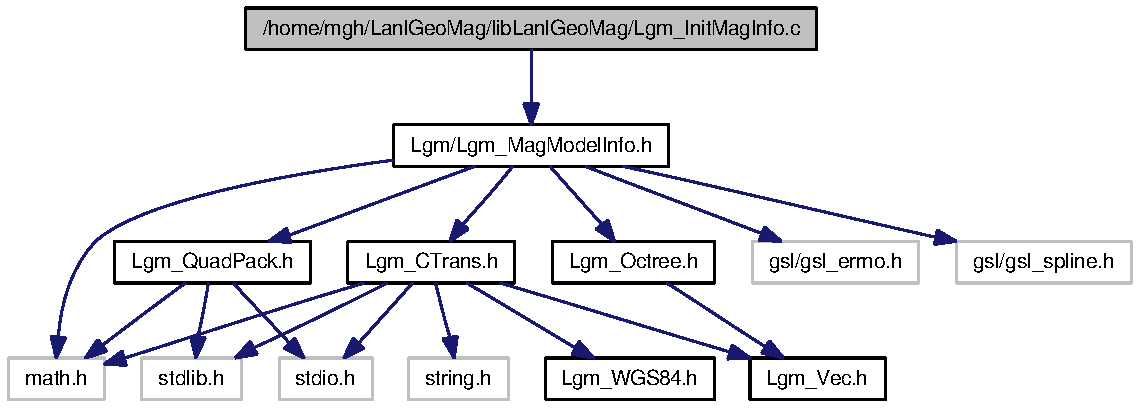
\includegraphics[width=291pt]{_lgm___init_mag_info_8c__incl}
\end{center}
\end{figure}
\subsection*{Functions}
\begin{CompactItemize}
\item 
\hyperlink{struct_lgm___mag_model_info}{Lgm\_\-MagModelInfo} $\ast$ \hyperlink{_lgm___init_mag_info_8c_4f16baeb21ae293220cd048d7bb8f757}{Lgm\_\-InitMagInfo} ()
\item 
void \hyperlink{_lgm___init_mag_info_8c_87ae57349dac55ae7393b6a168c080b2}{Lgm\_\-FreeMagInfo} (\hyperlink{struct_lgm___mag_model_info}{Lgm\_\-MagModelInfo} $\ast$Info)
\item 
\hyperlink{struct_lgm___mag_model_info}{Lgm\_\-MagModelInfo} $\ast$ \hyperlink{_lgm___init_mag_info_8c_d3b20a753c7c6d9afef944a6cf9880dc}{Lgm\_\-CopyMagInfo} (\hyperlink{struct_lgm___mag_model_info}{Lgm\_\-MagModelInfo} $\ast$s)
\item 
void \hyperlink{_lgm___init_mag_info_8c_1df3c4796964cae56b6c9bd883d5954b}{Lgm\_\-MagModelInfo\_\-Set\_\-Psw} (double Psw, \hyperlink{struct_lgm___mag_model_info}{Lgm\_\-MagModelInfo} $\ast$m)
\item 
void \hyperlink{_lgm___init_mag_info_8c_07ff6127e39836ffee154fe3b5eab5e9}{Lgm\_\-MagModelInfo\_\-Set\_\-Kp} (double Kp, \hyperlink{struct_lgm___mag_model_info}{Lgm\_\-MagModelInfo} $\ast$m)
\item 
void \hyperlink{_lgm___init_mag_info_8c_c318ccee75354e49cb61fe38ee8d82a4}{Lgm\_\-Set\_\-Octree\_\-kNN\_\-InterpMethod} (\hyperlink{struct_lgm___mag_model_info}{Lgm\_\-MagModelInfo} $\ast$m, int Method)
\item 
void \hyperlink{_lgm___init_mag_info_8c_678acc89e6dd0a339e73cd0016d182a8}{Lgm\_\-Set\_\-Octree\_\-kNN\_\-k} (\hyperlink{struct_lgm___mag_model_info}{Lgm\_\-MagModelInfo} $\ast$m, int k)
\item 
void \hyperlink{_lgm___init_mag_info_8c_dbde452adbe800b5292798a1668dd255}{Lgm\_\-Set\_\-Octree\_\-kNN\_\-MaxDist} (\hyperlink{struct_lgm___mag_model_info}{Lgm\_\-MagModelInfo} $\ast$m, double MaxDist)
\item 
void \hyperlink{_lgm___init_mag_info_8c_9df19c2b1d0c318e81e774c57ced1929}{Lgm\_\-Set\_\-Open\_\-Limits} (\hyperlink{struct_lgm___mag_model_info}{Lgm\_\-MagModelInfo} $\ast$m, double xmin, double xmax, double ymin, double ymax, double zmin, double zmax)
\end{CompactItemize}


\subsection{Function Documentation}
\hypertarget{_lgm___init_mag_info_8c_4f16baeb21ae293220cd048d7bb8f757}{
\index{Lgm\_\-InitMagInfo.c@{Lgm\_\-InitMagInfo.c}!Lgm\_\-InitMagInfo@{Lgm\_\-InitMagInfo}}
\index{Lgm\_\-InitMagInfo@{Lgm\_\-InitMagInfo}!Lgm_InitMagInfo.c@{Lgm\_\-InitMagInfo.c}}
\subsubsection[{Lgm\_\-InitMagInfo}]{\setlength{\rightskip}{0pt plus 5cm}{\bf Lgm\_\-MagModelInfo}$\ast$ Lgm\_\-InitMagInfo ()}}
\label{_lgm___init_mag_info_8c_4f16baeb21ae293220cd048d7bb8f757}




Definition at line 8 of file Lgm\_\-InitMagInfo.c.

Here is the call graph for this function:\nopagebreak
\begin{figure}[H]
\begin{center}
\leavevmode
\includegraphics[width=285pt]{_lgm___init_mag_info_8c_4f16baeb21ae293220cd048d7bb8f757_cgraph}
\end{center}
\end{figure}


Here is the caller graph for this function:\nopagebreak
\begin{figure}[H]
\begin{center}
\leavevmode
\includegraphics[width=197pt]{_lgm___init_mag_info_8c_4f16baeb21ae293220cd048d7bb8f757_icgraph}
\end{center}
\end{figure}
\hypertarget{_lgm___init_mag_info_8c_87ae57349dac55ae7393b6a168c080b2}{
\index{Lgm\_\-InitMagInfo.c@{Lgm\_\-InitMagInfo.c}!Lgm\_\-FreeMagInfo@{Lgm\_\-FreeMagInfo}}
\index{Lgm\_\-FreeMagInfo@{Lgm\_\-FreeMagInfo}!Lgm_InitMagInfo.c@{Lgm\_\-InitMagInfo.c}}
\subsubsection[{Lgm\_\-FreeMagInfo}]{\setlength{\rightskip}{0pt plus 5cm}void Lgm\_\-FreeMagInfo ({\bf Lgm\_\-MagModelInfo} $\ast$ {\em Info})}}
\label{_lgm___init_mag_info_8c_87ae57349dac55ae7393b6a168c080b2}




Definition at line 75 of file Lgm\_\-InitMagInfo.c.

Here is the call graph for this function:\nopagebreak
\begin{figure}[H]
\begin{center}
\leavevmode
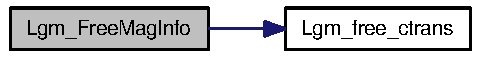
\includegraphics[width=133pt]{_lgm___init_mag_info_8c_87ae57349dac55ae7393b6a168c080b2_cgraph}
\end{center}
\end{figure}


Here is the caller graph for this function:\nopagebreak
\begin{figure}[H]
\begin{center}
\leavevmode
\includegraphics[width=206pt]{_lgm___init_mag_info_8c_87ae57349dac55ae7393b6a168c080b2_icgraph}
\end{center}
\end{figure}
\hypertarget{_lgm___init_mag_info_8c_d3b20a753c7c6d9afef944a6cf9880dc}{
\index{Lgm\_\-InitMagInfo.c@{Lgm\_\-InitMagInfo.c}!Lgm\_\-CopyMagInfo@{Lgm\_\-CopyMagInfo}}
\index{Lgm\_\-CopyMagInfo@{Lgm\_\-CopyMagInfo}!Lgm_InitMagInfo.c@{Lgm\_\-InitMagInfo.c}}
\subsubsection[{Lgm\_\-CopyMagInfo}]{\setlength{\rightskip}{0pt plus 5cm}{\bf Lgm\_\-MagModelInfo}$\ast$ Lgm\_\-CopyMagInfo ({\bf Lgm\_\-MagModelInfo} $\ast$ {\em s})}}
\label{_lgm___init_mag_info_8c_d3b20a753c7c6d9afef944a6cf9880dc}




Definition at line 90 of file Lgm\_\-InitMagInfo.c.

Here is the call graph for this function:\nopagebreak
\begin{figure}[H]
\begin{center}
\leavevmode
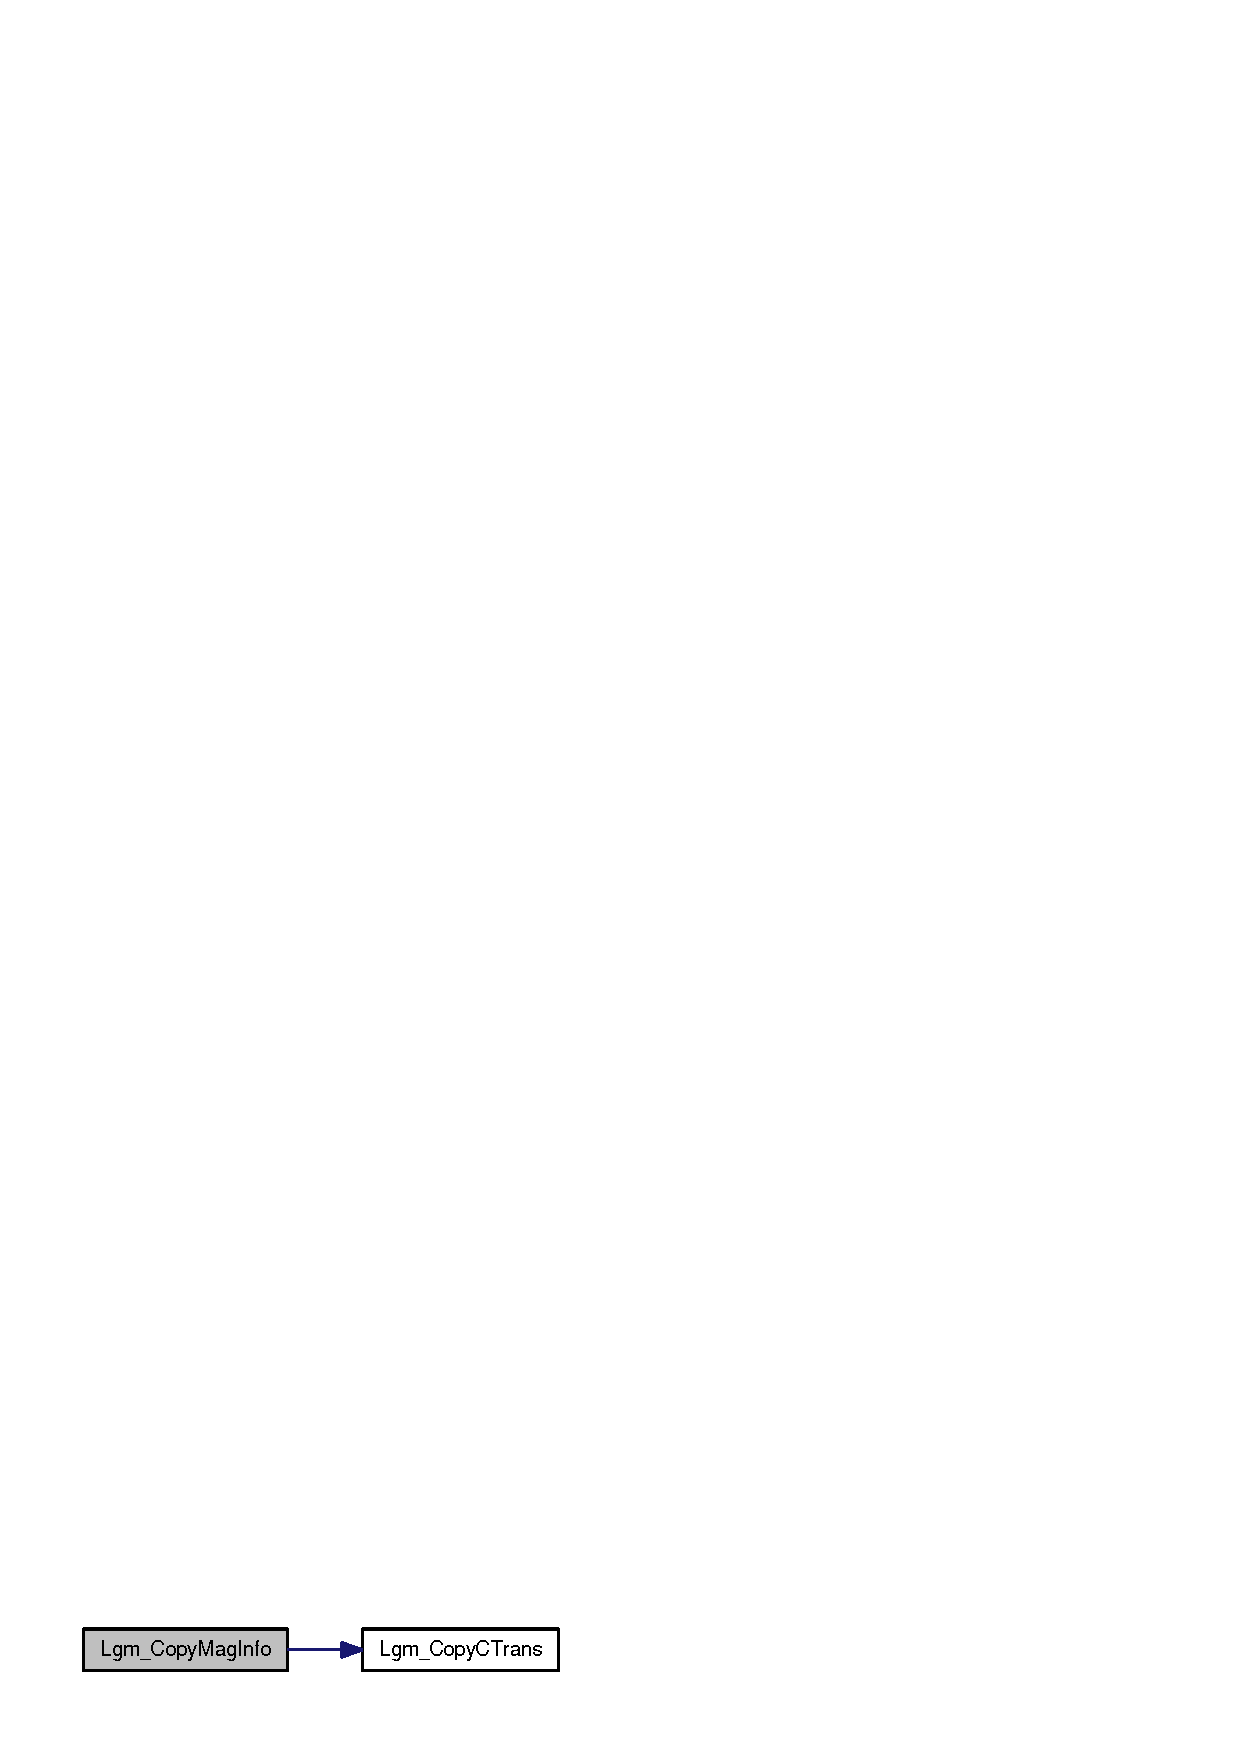
\includegraphics[width=136pt]{_lgm___init_mag_info_8c_d3b20a753c7c6d9afef944a6cf9880dc_cgraph}
\end{center}
\end{figure}


Here is the caller graph for this function:\nopagebreak
\begin{figure}[H]
\begin{center}
\leavevmode
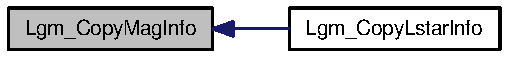
\includegraphics[width=140pt]{_lgm___init_mag_info_8c_d3b20a753c7c6d9afef944a6cf9880dc_icgraph}
\end{center}
\end{figure}
\hypertarget{_lgm___init_mag_info_8c_1df3c4796964cae56b6c9bd883d5954b}{
\index{Lgm\_\-InitMagInfo.c@{Lgm\_\-InitMagInfo.c}!Lgm\_\-MagModelInfo\_\-Set\_\-Psw@{Lgm\_\-MagModelInfo\_\-Set\_\-Psw}}
\index{Lgm\_\-MagModelInfo\_\-Set\_\-Psw@{Lgm\_\-MagModelInfo\_\-Set\_\-Psw}!Lgm_InitMagInfo.c@{Lgm\_\-InitMagInfo.c}}
\subsubsection[{Lgm\_\-MagModelInfo\_\-Set\_\-Psw}]{\setlength{\rightskip}{0pt plus 5cm}void Lgm\_\-MagModelInfo\_\-Set\_\-Psw (double {\em Psw}, \/  {\bf Lgm\_\-MagModelInfo} $\ast$ {\em m})}}
\label{_lgm___init_mag_info_8c_1df3c4796964cae56b6c9bd883d5954b}




Definition at line 129 of file Lgm\_\-InitMagInfo.c.\hypertarget{_lgm___init_mag_info_8c_07ff6127e39836ffee154fe3b5eab5e9}{
\index{Lgm\_\-InitMagInfo.c@{Lgm\_\-InitMagInfo.c}!Lgm\_\-MagModelInfo\_\-Set\_\-Kp@{Lgm\_\-MagModelInfo\_\-Set\_\-Kp}}
\index{Lgm\_\-MagModelInfo\_\-Set\_\-Kp@{Lgm\_\-MagModelInfo\_\-Set\_\-Kp}!Lgm_InitMagInfo.c@{Lgm\_\-InitMagInfo.c}}
\subsubsection[{Lgm\_\-MagModelInfo\_\-Set\_\-Kp}]{\setlength{\rightskip}{0pt plus 5cm}void Lgm\_\-MagModelInfo\_\-Set\_\-Kp (double {\em Kp}, \/  {\bf Lgm\_\-MagModelInfo} $\ast$ {\em m})}}
\label{_lgm___init_mag_info_8c_07ff6127e39836ffee154fe3b5eab5e9}




Definition at line 132 of file Lgm\_\-InitMagInfo.c.\hypertarget{_lgm___init_mag_info_8c_c318ccee75354e49cb61fe38ee8d82a4}{
\index{Lgm\_\-InitMagInfo.c@{Lgm\_\-InitMagInfo.c}!Lgm\_\-Set\_\-Octree\_\-kNN\_\-InterpMethod@{Lgm\_\-Set\_\-Octree\_\-kNN\_\-InterpMethod}}
\index{Lgm\_\-Set\_\-Octree\_\-kNN\_\-InterpMethod@{Lgm\_\-Set\_\-Octree\_\-kNN\_\-InterpMethod}!Lgm_InitMagInfo.c@{Lgm\_\-InitMagInfo.c}}
\subsubsection[{Lgm\_\-Set\_\-Octree\_\-kNN\_\-InterpMethod}]{\setlength{\rightskip}{0pt plus 5cm}void Lgm\_\-Set\_\-Octree\_\-kNN\_\-InterpMethod ({\bf Lgm\_\-MagModelInfo} $\ast$ {\em m}, \/  int {\em Method})}}
\label{_lgm___init_mag_info_8c_c318ccee75354e49cb61fe38ee8d82a4}




Definition at line 139 of file Lgm\_\-InitMagInfo.c.\hypertarget{_lgm___init_mag_info_8c_678acc89e6dd0a339e73cd0016d182a8}{
\index{Lgm\_\-InitMagInfo.c@{Lgm\_\-InitMagInfo.c}!Lgm\_\-Set\_\-Octree\_\-kNN\_\-k@{Lgm\_\-Set\_\-Octree\_\-kNN\_\-k}}
\index{Lgm\_\-Set\_\-Octree\_\-kNN\_\-k@{Lgm\_\-Set\_\-Octree\_\-kNN\_\-k}!Lgm_InitMagInfo.c@{Lgm\_\-InitMagInfo.c}}
\subsubsection[{Lgm\_\-Set\_\-Octree\_\-kNN\_\-k}]{\setlength{\rightskip}{0pt plus 5cm}void Lgm\_\-Set\_\-Octree\_\-kNN\_\-k ({\bf Lgm\_\-MagModelInfo} $\ast$ {\em m}, \/  int {\em k})}}
\label{_lgm___init_mag_info_8c_678acc89e6dd0a339e73cd0016d182a8}




Definition at line 143 of file Lgm\_\-InitMagInfo.c.\hypertarget{_lgm___init_mag_info_8c_dbde452adbe800b5292798a1668dd255}{
\index{Lgm\_\-InitMagInfo.c@{Lgm\_\-InitMagInfo.c}!Lgm\_\-Set\_\-Octree\_\-kNN\_\-MaxDist@{Lgm\_\-Set\_\-Octree\_\-kNN\_\-MaxDist}}
\index{Lgm\_\-Set\_\-Octree\_\-kNN\_\-MaxDist@{Lgm\_\-Set\_\-Octree\_\-kNN\_\-MaxDist}!Lgm_InitMagInfo.c@{Lgm\_\-InitMagInfo.c}}
\subsubsection[{Lgm\_\-Set\_\-Octree\_\-kNN\_\-MaxDist}]{\setlength{\rightskip}{0pt plus 5cm}void Lgm\_\-Set\_\-Octree\_\-kNN\_\-MaxDist ({\bf Lgm\_\-MagModelInfo} $\ast$ {\em m}, \/  double {\em MaxDist})}}
\label{_lgm___init_mag_info_8c_dbde452adbe800b5292798a1668dd255}




Definition at line 147 of file Lgm\_\-InitMagInfo.c.\hypertarget{_lgm___init_mag_info_8c_9df19c2b1d0c318e81e774c57ced1929}{
\index{Lgm\_\-InitMagInfo.c@{Lgm\_\-InitMagInfo.c}!Lgm\_\-Set\_\-Open\_\-Limits@{Lgm\_\-Set\_\-Open\_\-Limits}}
\index{Lgm\_\-Set\_\-Open\_\-Limits@{Lgm\_\-Set\_\-Open\_\-Limits}!Lgm_InitMagInfo.c@{Lgm\_\-InitMagInfo.c}}
\subsubsection[{Lgm\_\-Set\_\-Open\_\-Limits}]{\setlength{\rightskip}{0pt plus 5cm}void Lgm\_\-Set\_\-Open\_\-Limits ({\bf Lgm\_\-MagModelInfo} $\ast$ {\em m}, \/  double {\em xmin}, \/  double {\em xmax}, \/  double {\em ymin}, \/  double {\em ymax}, \/  double {\em zmin}, \/  double {\em zmax})}}
\label{_lgm___init_mag_info_8c_9df19c2b1d0c318e81e774c57ced1929}




Definition at line 153 of file Lgm\_\-InitMagInfo.c.

Here is the caller graph for this function:\nopagebreak
\begin{figure}[H]
\begin{center}
\leavevmode
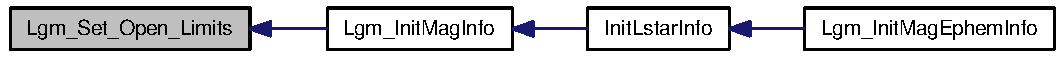
\includegraphics[width=273pt]{_lgm___init_mag_info_8c_9df19c2b1d0c318e81e774c57ced1929_icgraph}
\end{center}
\end{figure}
